\documentclass[12pt,a4paper]{report}
\usepackage{geometry}
\usepackage{tabularx}
\usepackage{booktabs}
\usepackage{amssymb}
\usepackage{subfigure}
\usepackage{multicol}
\geometry{
	a4paper,
	total={170mm,257mm},
	left=2.5cm,
	top=2.5cm,
	right=1.25cm,
	bottom=1.25cm
}
\usepackage[pdftex]{graphicx}
\usepackage{url} 
\usepackage[T1]{fontenc}
\usepackage{charter}

\usepackage[bookmarks, colorlinks=false, pdfborder={0 0 0}, pdftitle={<pdf title here>}, pdfauthor={<author's name here>}, pdfsubject={<subject here>}, pdfkeywords={<keywords here>}]{hyperref} 

\usepackage{listings}
\usepackage{xcolor}
\definecolor{codegreen}{rgb}{0,0.6,0}
\definecolor{codegray}{rgb}{0.5,0.5,0.5}
\definecolor{codepurple}{rgb}{0.58,0,0.82}
\definecolor{backcolour}{rgb}{0.95,0.95,0.92}
\rmfamily

\setcounter{secnumdepth}{5} % seting level of numbering (default for "report" is 3). With ''-1'' you have non number also for chapters
 %\setcounter{tocdepth}{5} % if you want all the levels in your table of contents
 
\lstdefinestyle{mystyle}{
    framesep=19pt,
	backgroundcolor=\color{backcolour},   
	commentstyle=\color{codegreen},
	keywordstyle=\color{magenta},
	numberstyle=\tiny\color{codegray},
	stringstyle=\color{codepurple},
	basicstyle=\mdseries\small,
	breakatwhitespace=false,         
	breaklines=true,                 
	captionpos=b,  
	basicstyle=\small,                
	keepspaces=true,                 
% 	numbers=left,                    
	numbersep=5pt,                  
	showspaces=false,                
	showstringspaces=false,
	showtabs=false,                  
	tabsize=2
}

\lstset{style=mystyle}
\begin{document}
\renewcommand\bibname{References} 
\begin{titlepage}    
    \begin{center}
        % \vspace{50cm}
        ~\\[2cm]
        
\includegraphics[width=6cm]{figures/gneLogo.png}\\[0.5cm]
        \huge{ Guru Nanak Dev Engineering College, Ludhiana}\\[0.5cm]
        \LARGE{Department of Computer Science and Engineering}\\[2cm]
        \linespread{1.2}\huge {
            Project Report of Artificial Intelligence Laboratory\\
            \large{( LPCCS-106 )}
        }
        \linespread{1}~\\[2cm]
        
        \begin{multicols}{2}
            
            {\large 
                \emph{Submitted To:} \\
            }
            {\large 
                Prof. Manpreet Kaur Mand
            }
            
            \columnbreak
        
            {\large 
                \emph{Submitted By:}\\[0.5cm]
            }
            {\large 
                Amanjot Singh - 2004691\\
                Priyanka Jhamb - 1905379\\
                Vrishti Gupta - 1905064\\[2cm]
            }
            
        \end{multicols}
        \vfill
        \linespread{0.5}~\\[0.5cm]
    \end{center}
\end{titlepage}
\pagenumbering{roman}
\tableofcontents
\newpage
\pagenumbering{arabic} 
\chapter{Tic Tac Toe Game}
\section{Introduction}
"Tic Tac Toe" is a AI Single-Player game played by a Player and computer on a 3x3 board.
The computer will choose a random position on the board to place its mark.
The Player can then place their mark on the board.
The Player can then choose to play again or exit the game.
The Player can also see his/her score, wins, loses.
\section{Tech Stack}
\label{Tech_Stack}
\subsection{SQL}
SQL is a database computer language designed for the retrieval and management of data in a relational database. SQL stands for Structured Query Language. The uses of SQL include modifying database table and index structures; adding, updating and deleting rows of data
\subsection{Python}
Python is a general-purpose interpreted, interactive, object-oriented, and high-level programming language. 
\subsection{Tkinter}
Python offers multiple options for developing GUI (Graphical User Interface). Out of all the GUI methods, tkinter is the most commonly used method. It is a standard Python interface to the Tk GUI toolkit shipped with Python. Python with tkinter is the fastest and easiest way to create the GUI applications. Creating a GUI using tkinter is an easy task.

\chapter{Project}
\section{Project Flow }
\begin{enumerate}
    \item Importing Required Libraries.
        \subitem os 
        \subitem random
        \subitem sqlite3
        \subitem time
        \subitem tkinter
        \subitem deepcopy
        \subitem partial
        \subitem PIL
        \subitem font
        \subitem pyglet
    \item Splash Page will appear.
    \item First Screen having asking Player's name and Option of Play as well as Link to the Developers Page will show.
    \item Second Screen having board of game.
    \item Then Player will play.
    \item Result Screen will be displayed in which game result, option of play game again and exit option. 
\end{enumerate}

\section{Program}
\lstinputlisting[language=Python,style=mystyle, label=chapters/code/tic tac toe.py]{chapters/code/tic tac toe.py}

\section{Output}

\hspace{14pt}
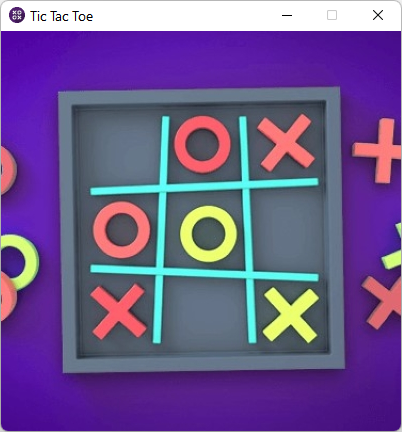
\includegraphics[width=8cm, height=9cm]{figures/splash_page.png}
\hfill
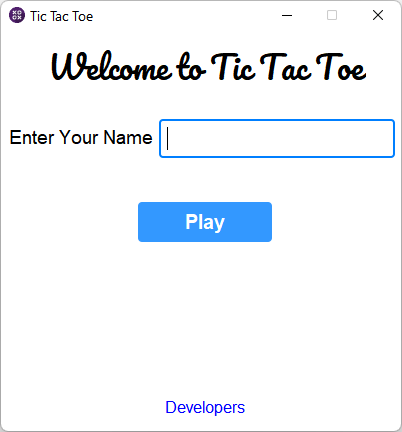
\includegraphics[width=8cm, height=9cm]{figures/first_screen.png}

\vspace{15pt}

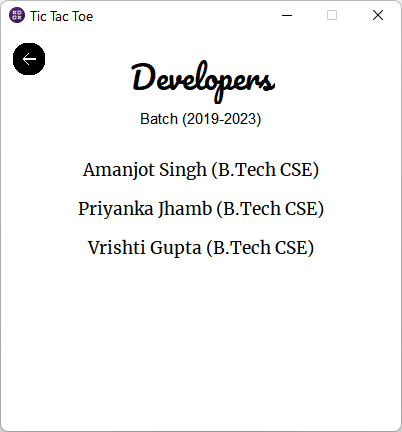
\includegraphics[width=8cm, height=9cm]{figures/developers_page.png}
\hfill
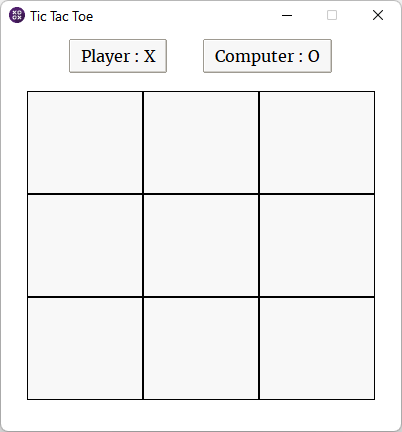
\includegraphics[width=8cm, height=9cm]{figures/GameBoard_page.png}

\vspace{10pt}

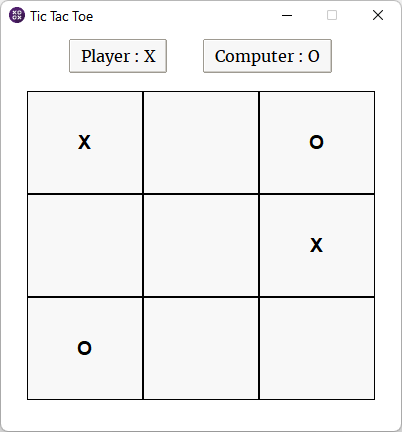
\includegraphics[height=8cm, width=8cm]{figures/GameBoard_page2.png}
\hfill
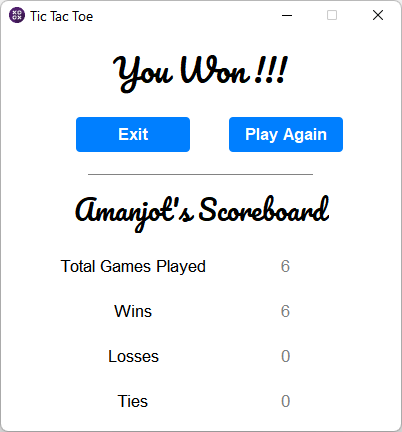
\includegraphics[height=8cm, width=8cm]{figures/Result_page_player_win.png}

\vspace{10pt}

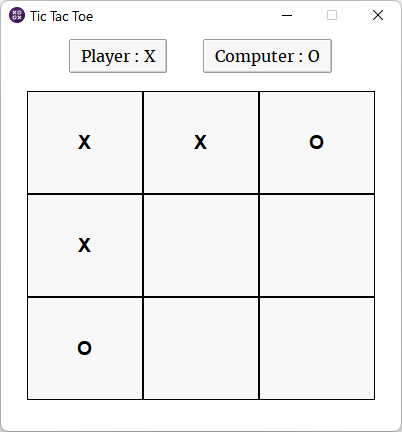
\includegraphics[height=8cm, width=8cm]{figures/GameBoard_page3.png}
\hfill
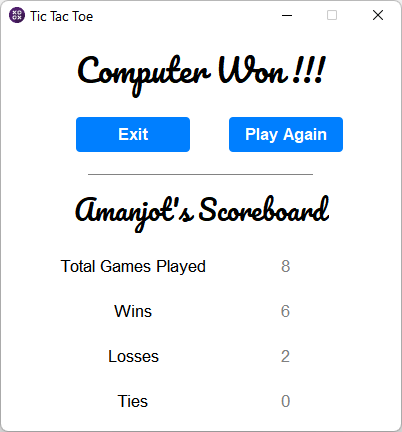
\includegraphics[height=8cm, width=8cm]{figures/Result_page_computer_win.png}

\vspace{15pt}
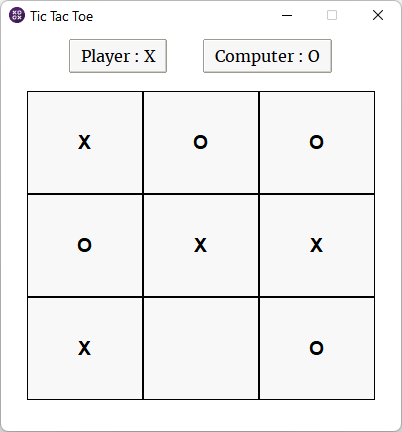
\includegraphics[height=8cm, width=8cm]{figures/GameBoard_page_tie.png}
\hfill
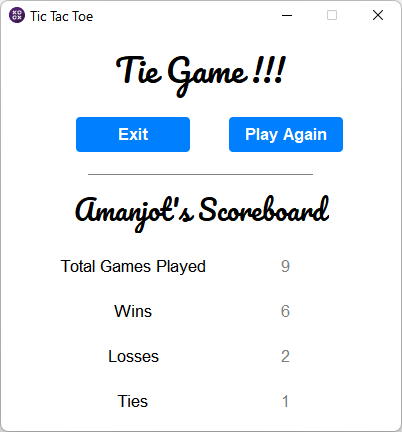
\includegraphics[height=8cm, width=8cm]{figures/Result_page_tie.png}

\chapter{Conclusion}

\hspace{1cm}Flutter is one of the most innovative mobile technologies on the market right now. For businesses looking to create applications on both iOS and Android, Flutter is a great option. If you are seeking apps with amazing UI and high performance — Flutter is the best option as well.\\\\

Flutter is not a universal remedy for everything, but it is a 100 percent promising framework, considering the breadth of coverage and speed of implementation. If you are looking for a team of Flutter experts, hesitating whether or not Flutter is the best option for you right now, or have any questions left after reading the article — our specialists are ready to consult with you on all these topics.\\\\

Flutter framework does a great job by providing an excellent framework to build mobile applications in a truly platform independent way. By providing simplicity in the development process, high performance in the resulting mobile application, rich and relevant user interface for both Android and iOS platform, Flutter framework will surely enable a lot of new developers to develop high performance and feature-full mobile application in the near future.

\newpage
\section{References}

[1] Timothy Arndt and Angela Guercio. Blockchain-based transcripts for mobile higher-
education. International Journal of Information and Education Technology, 10:84–89,
01 2020
\\

\noindent[2] Sura I. Mohammed Ali, Haitham Farouk, and Hussien Sharaf. A blockchain-based
models for student information systems. Egyptian Informatics Journal, 2021
\\

\noindent[3] Antonio Bartolomé, Carles Torlà, Linda Castañeda, and Jordi Adell. Blockchain in
education: Introduction and critical review of the state of the art. 61, 01 2017.
\\

\noindent[4] Benjamin W Cashman Richard S. Clark Ronald P. Uhlig, Rich Yonts and Brett Niema, Blockchain in Education: Introduction and Critical Review of the State of the Art, 2017
\\

\noindent[5] Blockchain Course: https://www.udemy.com/course/build-your-blockchain-az/
\\

\noindent[6] Proof of authority Online Material: 
\begin{itemize}
    \item Wikipedia, 
    \item https://academy.binance.com/en/articles/proof-of-authority-explained ,
\end{itemize}

  
% \href{https://en.wikipedia.org/wiki/Proof\_of\_authority#:~:text=Proof\%20of\%20authority\%20(PoA)\%20is,platform\%20using\%20PoA\%20is\%20VeChain.}{https://en.wikipedia.org/wiki/Proof_of_authority#:~:text=Proof\%20of\%20authority\%20(PoA)\%20is,platform\%20using\%20PoA\%20is\%20VeChain.}

\noindent[7] IPFS Documentation: https://ipfs.io/ \\

\noindent[8] https://medium.com/python-pandemonium/getting-started-with-python-and-ipfs-94d14fdffd10
\\

% \noindent[8] Github Projects 

% \cite{ALI2021}
% \cite{article}
% \cite{asee_peer_31816}
% \cite{article12}
% \bibliographystyle{plain}
% \bibliography{1.bib}
\end{document}
